\subsection{模型综述}
\subsubsection{模型背景}
在之前的模型设计当中,我们从冷启动和高阶特征提取上对于模型进行了设计。在经过一系列训练和测试之后,我们对于我们的模型进行了一定的修正和调整,最后确定模型名称为Combining Explicit and Implicit Feature Interaction between Users and Items with Multi-Head Attention。本模型主要处理了两种推荐系统中存在的问题或者特性:

首先是时效性。在当前的信息爆炸的时代,每天都有海量的数据被上传到互联网上,这些新上传的数据很难在开始时取得足够量的评分数据,被用于推荐系统中进行面向目标用户的推荐。一个较为典型的例子是新闻推荐系统。每天都有各种主题的新闻被上传,保证推荐新闻的时效性也是新闻推荐系统的一个重要的条件。音乐推荐系统也是如此,经常会有一些新歌发售,需要推荐给用户来进行试听。所以我们通过模型的冷启动机制,解决这样新内容推荐的问题。使得推荐系统能够应对时效性和新内容带来的问题。

再有是个性化。我们认为用户在评价歌曲时,就算两个人对于同一首歌都给出了喜欢的评价,但是他们的动机可能是不同的,比如说一个人喜欢歌手所以喜欢这首歌,另一个人喜欢这首歌的歌曲风格而喜欢这首歌。从而,模型需要对于歌曲的推荐进行更加富有个性化的处理,更好地对于音乐特征和用户特征进行个性化的处理。

依据上面的背景问题,我们对于以前的相关系统的性能进行了讨论。

\subsubsection{以往模型的问题}
在以往的模型中,我们发现一个问题是对于内容(在音乐推荐中指音乐)的编码。编码过程中,并没有使用到于其交互的用户的信息。这就导致了用户个性在推荐内容上的缺失,相同的内容即使对于不同的两个用户,其编码还是相同的,这就不能很好地处理我们上面提出的个性化的问题。

此外,在实际的交互过程中,内容和用户有不同的交互行为,不同的交互行为往往代表用户的喜好程度不一,而以往的模型并不对这种程度上的不同进行区分,这就导致不同交互行为带来的不同信息没有被使用。例如对于点赞和收藏两种行为,收藏表示用户的兴趣程度要高于点赞,因为收藏意为着用户很有可能会在之后重复听这首歌曲,而点赞不会有这种行为。

\subsubsection{形式化描述}
\begin{itemize}
    \item 用户:$U=\{field_{1}^{u}, field_{2}^{u}, \cdots, field_{n_u}^{u}\}$表示用户的相关特征信息
    \item 待判断音乐:$M=\{field_{1}^{m}, field_{2}^{m}, \cdots, field_{n_m}^{m}$表示音乐的相关特征信息
    \item 用户$U$的历史交互数据:$H=\{M_1', M_2',\cdots, M_k'\}$,其中对于音乐$M_i‘$的评分为$score_i$
    \item 标签$y=0/1$,$0$表示不喜欢,$1$表示喜欢。
\end{itemize}

\subsubsection{模型结构}
\begin{figure}[htb]        
\center{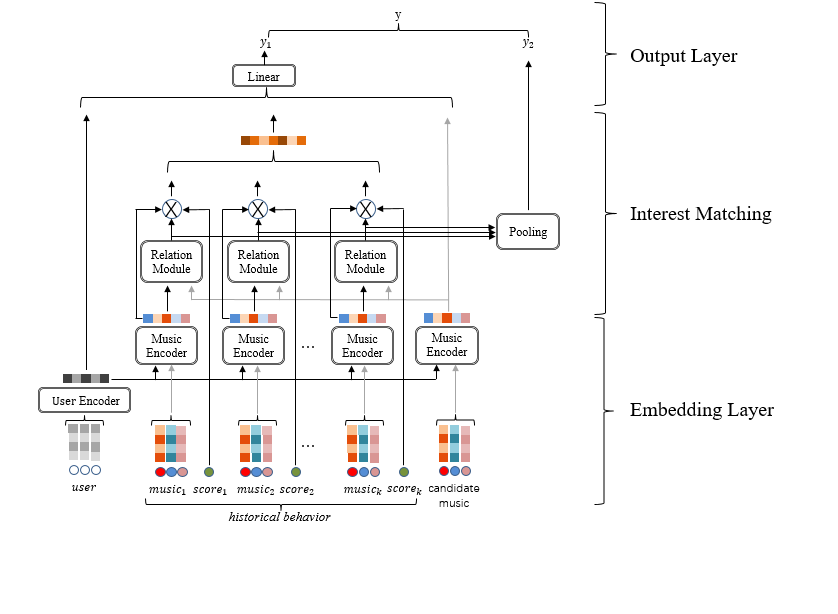
\includegraphics[width=15cm]  {MusicRecomSurvey/pics/model_final.PNG}}    
\caption{\label{4} 模型结构图}      
\end{figure}

详细的模型介绍将在之后的实验方案改进说明中给出。

\subsubsection{程序设计方案}
我们通过Python和PyTorch等开源库,搭建了我们的数据处理模块,以及神经网络结构。具体的设计思路在附录X中。